\documentclass[journal,12pt,twocolumn]{IEEEtran}
\usepackage{graphicx}
\graphicspath{{./figs/}}{}
\usepackage{amsmath,amssymb,amsfonts,amsthm}
\newcommand{\myvec}[1]{\ensuremath{\begin{pmatrix}#1\end{pmatrix}}}
\usepackage{listings}
\usepackage{watermark}
\usepackage{titlesec}
\let\vec\mathbf

\titlespacing{\subsection}{0pt}{\parskip}{-3pt}
\titlespacing{\subsubsection}{0pt}{\parskip}{-\parskip}
\titlespacing{\paragraph}{0pt}{\parskip}{\parskip}
\newcommand{\figuremacro}[5]{
    
}
\lstset{
frame=single, 
breaklines=true,
columns=fullflexible
}
\thiswatermark{\centering \put(0,-105.0){
\includegraphics[scale=0.08]{logo.jpg}} }

\sloppy
\title{\mytitle}
\title{
Matrix Assignment - Conic
}
\author{T.Sai Raghavendra(FWC22087)}
\begin{document}
\maketitle
\tableofcontents
\bigskip


\section{Problem}
If the line x-1=0 is the directrix of the parabola to $y^2-kx+8=0$ then find one of the values of k


\section{Solution}

we know that the vector equation of the line is 
\begin{align}
\label{eq:one}
\vec{n}^\top x = c
\end{align}

By comparing the given line with \eqref{eq:one} we get, 

\begin{center}
$\vec{n} = \myvec{1\\0}$ , c = 1 
\end{center}

\begin{align}
\label{eq:two}
\vec{y^2}-k\vec{x}+8=0 
\end{align}

We know that the equation of a conic with directrix $\vec{n}^\top x = c$, eccentricity e and focus F is given by 
\begin{align}
\label{eq:three}
\vec{x^\top Vx}+2\vec{u^\top}x+f = 0 
\end{align}


Compare the given parabola \eqref{eq:two} with \eqref{eq:three} we get,
\begin{center}
$\vec{V} = \myvec{0&0\\0&1}$ $\vec{u} = \myvec{\frac{-k}{2} \\ \\ 0}$ , f = 8
\end{center}

Finding the vector $\vec{u}$ we can obtain the k value, 

To find vector $\vec{u}$ we have,

\begin{align}
\label{eq:four}
\vec{u}=ce^2\vec{n}-||\vec{n}||^2\vec{F}
\end{align}
To find Focus $\vec{F}$ in \eqref{eq:four} we have,
\begin{align}
\label{eq:five}
\vec{F} = \frac{\frac{\eta}{4\sqrt{\lambda_2}}\sqrt{\lambda_2}e_1 - \frac{\eta}{2}e_1}{\lambda_2}
\end{align}

From the given parabola and line we have,
\begin{center}
$\lambda_2 =1$, c = 1, $\vec{e_1} = \myvec{1 \\ 0}$
\end{center}


$c = \frac{\eta}{4\sqrt{\lambda_2}}$ $\implies$ $\eta = 4.c.\lambda_2$ = 4\\

On substituting $\eta$,$\lambda_2$,$\vec{e_1}$ in \eqref{eq:five} we get,

\begin{center}
$\vec{F} = \myvec{-1 \\ 0}$
\end{center}

By substituting the $\vec{F}$,c,$\vec{e_1}$,$\vec{n}$ in \eqref{eq:four} we get,
\begin{center}
$\vec{u}$ = $\myvec{2 \\ 0}$
\end{center} 

Equating the vectors $\vec{u}$ we get,

\begin{center}
k = 4
\end{center}


\section{Figure}
\begin{figure}[h]
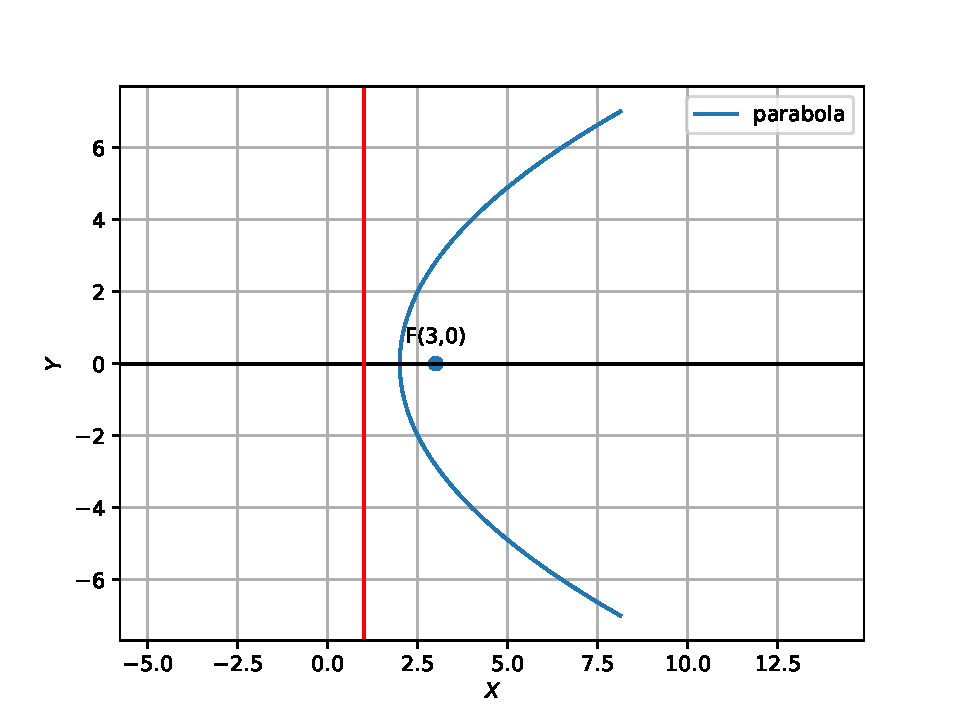
\includegraphics[width=\columnwidth]{fig.pdf}
\caption{To find the value of k and plotting the parabola}
    \label{fig:my_label}
\end{figure}


\begin{center}
$\vec{IV.\hspace{.2cm} Code Link}$
\end{center}
\begin{lstlisting}
https://github.com/Sairaghavendra36/Fwc-2022/blob/main/Matrices/Code/Conic.py
\end{lstlisting}
Execute the code by using the command
\textbf{python3 line.py}


\end{document}